% !TEX root = ../main.tex

\chapter{绪论}
\section{引言}
三维模型形状编辑是图形学及其相关领域中不可或缺的一部分,无论在研究还是工业领域都存在着广泛的需求和应用。在经历了空间变形、多分辨率变形、微分域变形等几个研究热点之后,这一领域已得到了较为成熟的发展。众多研究者提出了各种方法以针对不同的需求场景。

但是随着网络带宽的增加,硬件性能的提升,使得大众可以很方便的传输、显示较大的三维模型。自然,大众对于模型质量的要求也随之提高,随之而来的还有对高质量三维内容的需求。另一方面,VR/AR的兴起进一步加强这一需求。这些也对三维模型形状编辑算法提出了新的要求,如提高编辑后模型的质量以满足大众对于高质量模型的需求,改进交互方式以便用户快速的创作三维模型,提升算法的效率使得用户可以编辑更大的模型。

空间变形作为一类简易,高效的三维模型形状编辑方法,近年来也发展出了一些新的变种以应对上文中提到的要求,如基于GPU的FFD算法\cite{chua2000, modat2010}、精确自由变形\cite{Feng98, Feng00}、光滑自由变形\cite{Cui15}等。

本文的形容方向是自由变形,并在光滑自由变形\cite{Cui15}的基础上提出了一种改进的算法。

光滑自由变形使用了CUDA加速算法,并根据模型的法向信息对变形结果进行了调整,使得算法具有实时编辑,变形结果更加自然细腻的优势。但是由于CUDA只能的Nvidia的显卡上运行,所以Cui的这一工作也被限制在了Nvidia平台上。另一方面,为了使组成模型的面片在变形后为贝赛尔三角片,光滑自由变形在预处理阶段需要将面片沿节点盒切割。该步骤很可能会产生一些狭长的或者退化的三角形,这些三角形不仅会造成计算资源的浪费,还可能影响算法的稳定性。

本文针对上述光滑自由变形的两个不足,进行了一系列深入的研究,在介绍本文工作之前,让我们先来回顾一下前人的相关工作。

\section{相关工作}
在诸多三维模型形状编辑算法中,空间变形是一种出现时间比较早,应用比较广泛的算法框架。该方案的基本思想最初由Barr\cite{Barr84}在1984年提出。Sederberg\cite{Sederberg86}于1986提出了经典的自由变形(Free-Form Deformation, 简称FFD),将这一思想完善为一个成熟的算法框架:
\begin{enumerate}
	\item 定义一个变形空间,也可以称之为中间体。
    \item 将待变形的模型“嵌入”到变形空间中,即计算模型上的采样点在变形空间中的参数坐标,该坐标在变形过程中保持不变。\label{item:2}
	\item 对变形空间进行变形。\label{item:3}
    \item 根据\ref{item:2}中得到的参数坐标与\ref{item:3}中得到的新变形空间,重新计算出采样点在欧氏空间中的坐标,从而达到变形的目的。
\end{enumerate}

\begin{figure}[htbp]
	\centering
	\begin{subfigure}[b]{.4\textwidth}
		\centering
		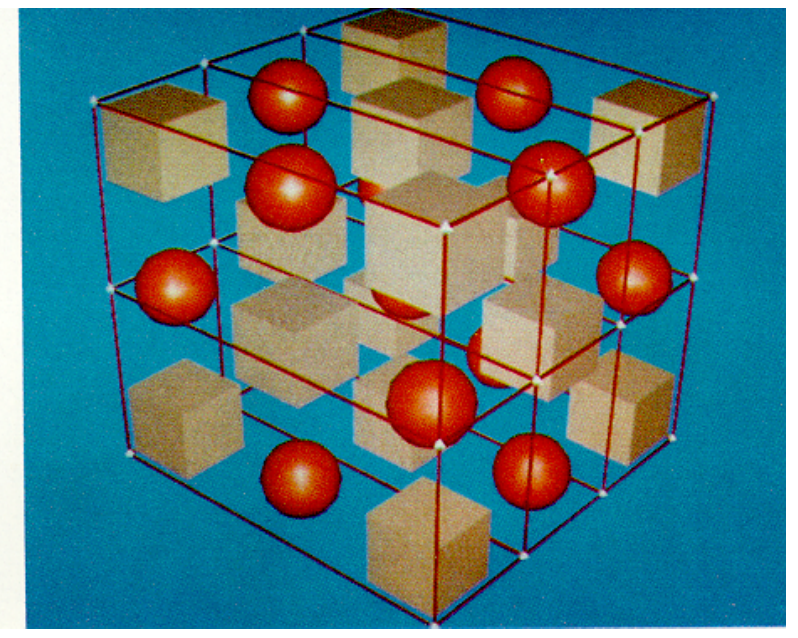
\includegraphics[width = \textwidth]{FFD_demo_0.png}
		\caption{原模型及中间体}\label{subfig:FFD_demo_0}
	\end{subfigure}
	\quad
	\begin{subfigure}[b]{.4\textwidth}
		\centering
		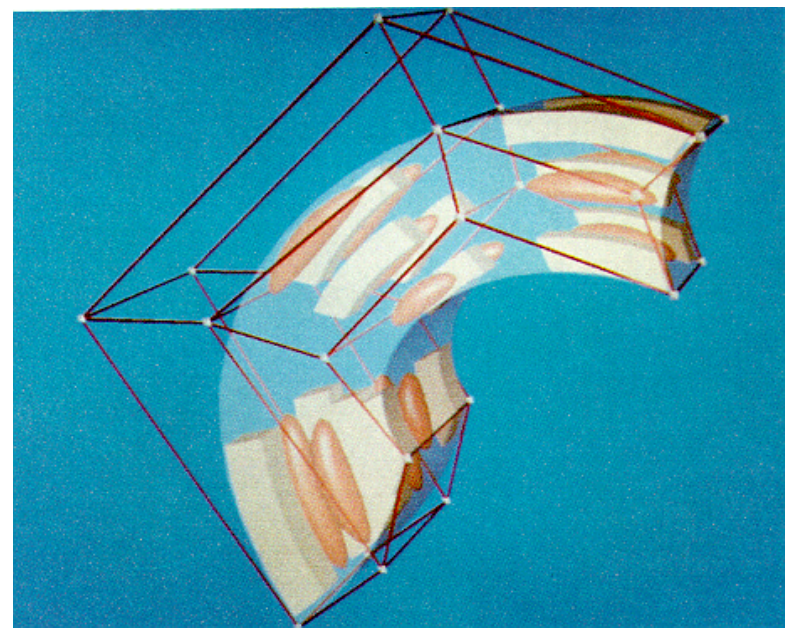
\includegraphics[width = \textwidth]{FFD_demo_1.png}
		\caption{FFD变形结果}\label{subfig:FFD_demo_1}
	\end{subfigure}
    \caption{自由变形示意图}\label{fig:FFD_demo}
\end{figure}

该方法具有直观、简单、高效的优点,很多学者在在此基础上提出了大量关于FFD算法的研究与改进。

中间体的选取是空间变形算法的关键,算法的效率、交互方式、变形结果等会因中间体表达方式的改变而改变。所以很多研究工作都着眼于中间体的改进:

Griessmair\cite{Griessmair89}和Lamousin\cite{lamousin1994}分别用B样条体和非均匀有理B样条体替换传统FFD\cite{Sederberg86}中的贝赛尔体,由于B样条体和非均匀有理B样条体的局部支撑性,使得模型的变形具有局部可调性。Coquillart\cite{coquillart1990}则通过移动、“焊接”长方体控制网格中的部分控制顶点,使得控制网格不再局限于长方体,而是将其转变圆柱等更加复杂的形状。这一改变虽然增加了变形模型嵌入变形空间过程中的计算量且对于控制网格的形状有一定的限制,但是改进了交互方式,使用户能够进行更为复杂的变形。

后续的学者进一步提出了以曲面、曲线甚至是以点为变形工具来构建变形空间。这些方法各自适用于不同的变形场合。如基于曲线的FFD适合基于骨架变形或者细长物体的变形,基于曲面的变形比较适用于形状较为扁平的模型的变形。总体而言,用户编辑模型时可以控制的变量越多,算法对模型的编辑能力就越强,能完成更加复杂的变形,但同时用户的交互也越复杂。在Gain和Beckmann的综述\cite{Gain08}中,作者对常见的FFD按照选用变形空间的不同进行了分类,并从局部可调性、交互友好度、时空效率、是否保拓扑等方面详细对比了各个方法的优劣。

上述这些方法中,无论中间体如何选择,用户都需要通过操作控制顶点来对中间体进行变形,中间体再通过采样点的参数坐标将变形“传导”到待变形的模型中。这一交互方式对普通用户而言并不友好,控制顶点的位移与待变形模型的顶点的位移并不完全一致。用户需对中间体的数学表示有所了解,才能实现复杂的变形意图。

为了解决这一问题,Hsu\cite{hsu1992}最先提出了直接自由变形,这一算法允许用户指定待变形模型上的一组点,并由用户提供这组点变形前后在欧氏空间中的位移。以前述信息为输入,算法将自动求出一组合适的控制顶点,使得用户指定的点的位移与输入保持一致。再由这组控制顶点求得最终变形结果。

随后,其它研究者也在此基础上提出了许多类似方法。这一类方法直接关联用户输入和变形结果,使用户直接编辑模型变形前后关键点的位置,即可等到整体的变形结果,而无需关心中间体的数学表示。使得FFD的交互更加便捷、直观。

传统FFD方法的另一个不足之处是变形过程中的走样问题。

由于传统FFd方法将变形是作用到待编辑模型的采样点上的,再由采样点变形后的位置,还原出模型的变形结果。所以,最终得到的变形结果的质量很大程度上依赖于采样点的密度。下\autoref{fig:sample_problem}很好的演示了这一问题。柜子的四个腿在原模型中由狭长的三角形组成,并且从视觉上看是与底部十字木条连在一起的。但是若以模型顶点为采样点,进行如\autoref{subfig:sample_problem_1}所示的变形后,柜子腿从视觉上与底部的十字木条分开了。这是由于采样点过于稀疏,变形只作用于柜子腿底部的顶点,而未作用于柜子腿与十字木条相连的部分造成的。

\begin{figure}[htbp]
	\centering
	\begin{subfigure}[b]{.4\textwidth}
		\centering
		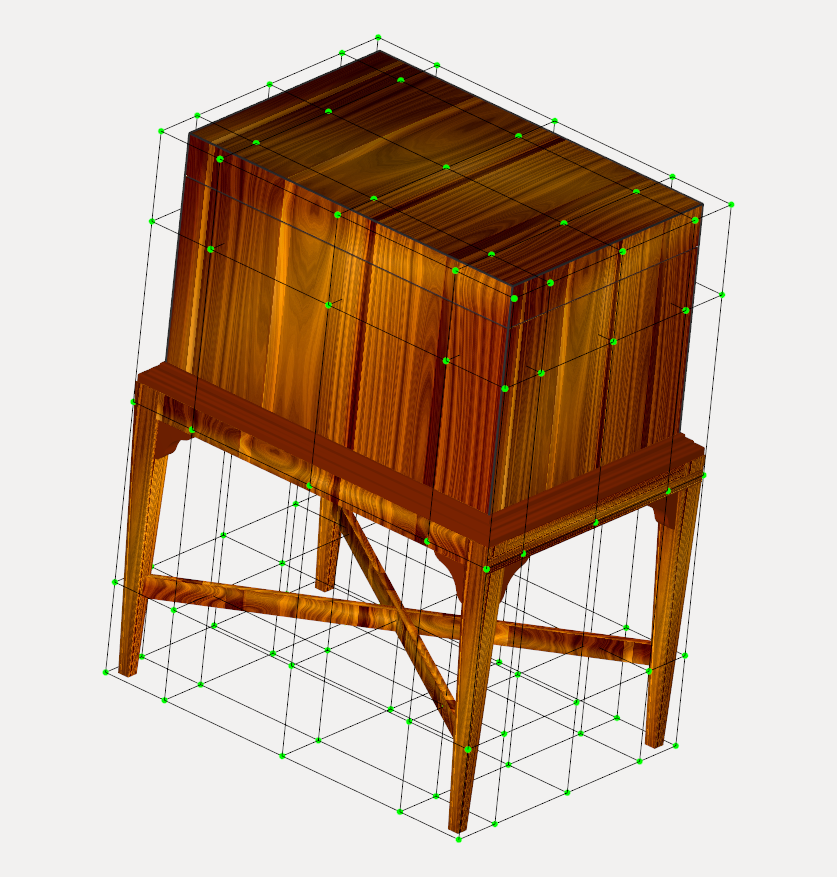
\includegraphics[width = \textwidth]{sample_problem_1.png}
		\caption{原模型}\label{subfig:sample_problem_0}
	\end{subfigure}
	\quad
	\begin{subfigure}[b]{.4\textwidth}
		\centering
		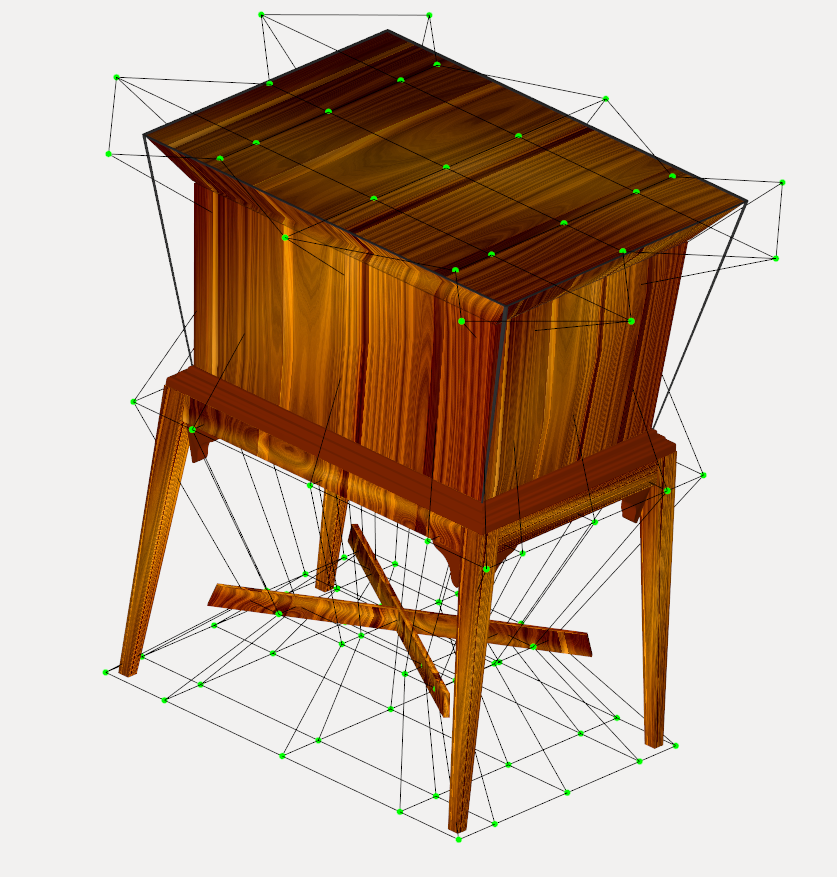
\includegraphics[width = \textwidth]{sample_problem_2.png}
		\caption{传统FFD变形结果}\label{subfig:sample_problem_1}
	\end{subfigure}
    \caption{传统FFD由于采样密度不足造成的精度问题}\label{fig:sample_problem}
\end{figure}

这一问题最直接的解决办法是通过均匀加密采样增加采样点的密度,但这一方法会造成性能上较大的开销。更进一步的方法\cite{parry1986, gain1999}是根据面片大小和曲面的曲率,自适应确定采样密度.自
适应采样虽然从性能上较之均匀加密采样有了较大的提升,但自适应算法实现相对复杂,并且无法很好的处理一些奇异情况。


为了更好的解决FFD中的走样问题,Feng\cite{Feng98}提出了“精确自由变形”。传统FFD是以采样点为变形对象的,而该方法以组成模型的曲面为变形对象的。变形算法的直接输出也不再是采样点变形后的位置,而是初始三角面片经由变形得到的新的曲面片。这样一来就避免了传统方法中采样过程所带来的走样问题。文中首先证明了:若自由变形采用的中/间体为B样条体,且待变形的三角面片位于唯一的节点盒之中\footnote{即三角面片只位于某个节点盒之内,而非跨节点盒},那么该三角面片的变形结果为一个三角贝赛尔曲面片,且其次数为B样条体三个维度上的次数之和。然后,作者再通过函数复合\cite{derose1988, derose1993}和位移算子\cite{chang1984},计算出三角贝赛尔曲面片的控制顶点,从而得到精确而自然的变形结果。\autoref{fig:sample_problem_affd}中对比了精确FFD与传统FFD的变形结果。

\begin{figure}[htbp]
	\centering
	\begin{subfigure}[b]{.3\textwidth}
		\centering
		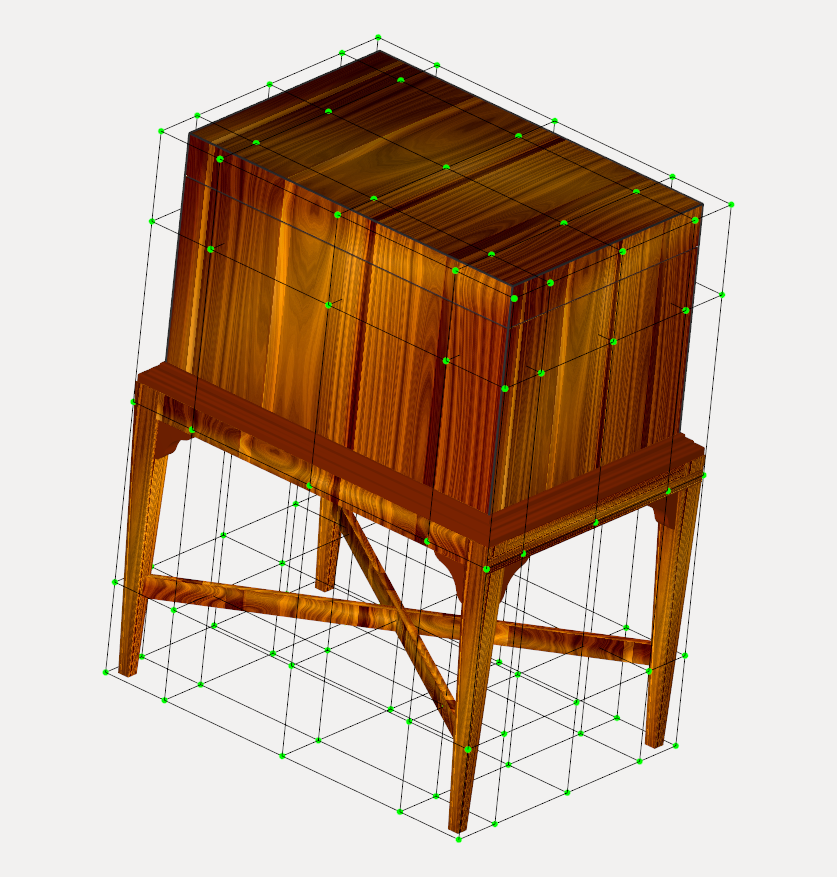
\includegraphics[width = \textwidth]{sample_problem_1.png}
		\caption{原模型}
	\end{subfigure}
	\quad
	\begin{subfigure}[b]{.3\textwidth}
		\centering
		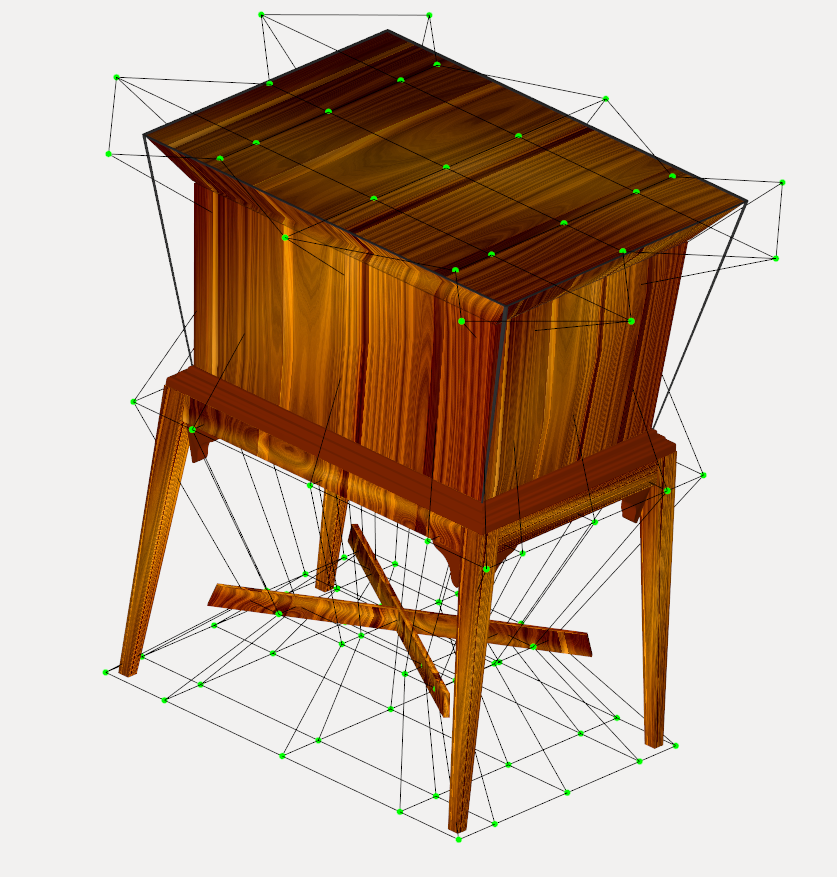
\includegraphics[width = \textwidth]{sample_problem_2.png}
		\caption{传统FFD变形结果}
	\end{subfigure}
	\quad
	\begin{subfigure}[b]{.3\textwidth}
		\centering
		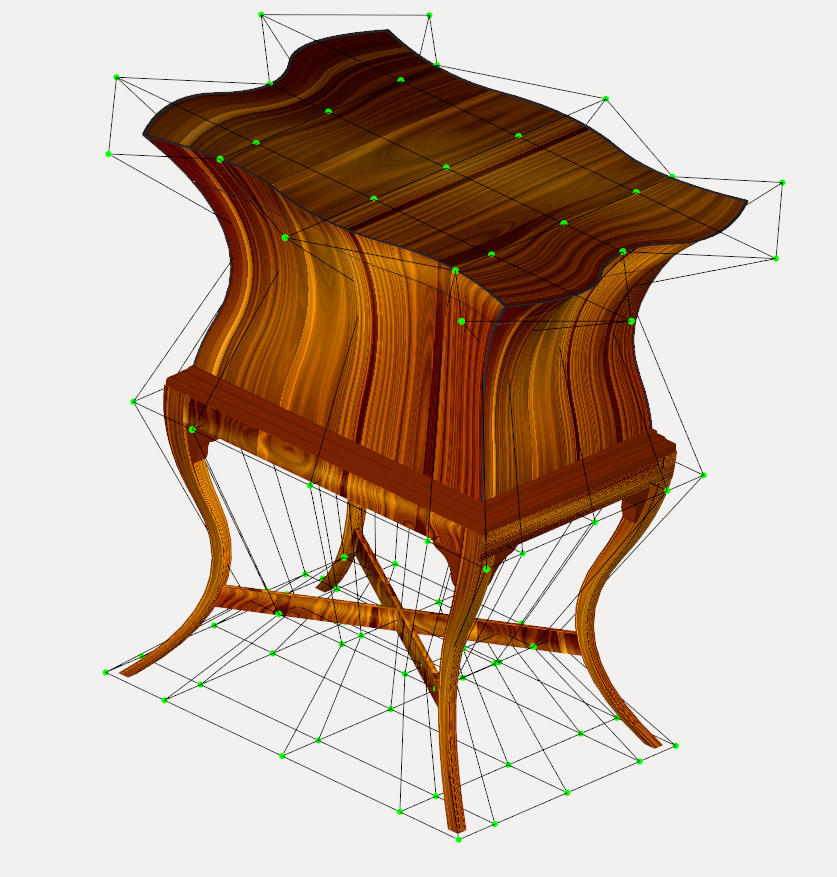
\includegraphics[width = \textwidth]{sample_problem_affd.png}
		\caption{精确FFD变形结果}
	\end{subfigure}
    \caption{传统FFD和精确FFD的结果对比}\label{fig:sample_problem_affd}
\end{figure}

作者在后续工作\cite{Feng00, Feng02}中对上述算法进行了改进,不仅使算法开销更低,还提升了算法的通用性。尽管如此,采用精确自由变形编辑较大的模型时,仍然无法做到实时交互。

另一方面,通用计算在近年来得到了较大的发展,GPU从一个仅负责图形绘制的专用硬件渐渐演变为一个多线程、高带宽的通用计算硬件。CUDA、OpenCL等通用计算框架的出现,更是进一步方便了应用程序利用GPU的强大的计算能力,以大幅提升其运行速度。FFD的构架下的算法大多是计算密集型的,且这些算法能较好的适用于单指令流多数据流计算模型,所以随着通用计算的兴起,自然有很多学者利用GPU加速各类FFD,从而使这些算法能对大型三维模型进行实时编辑。

其中,Cui\cite{Cui13}的工作成功地将CUDA应用到了精确自由变形中,采用GPU实现的算法相较于原先的CPU版本快了50倍左右。另一方面,无论是传统的FFD还是精确FFD,在其变形过程中都只考虑了待变形的模型的几何信息,而未考虑模型的法向信息。所以变形之后得到的模型会有不光滑的走样,\autoref{subfig:saffd_0}和\autoref{subfig:saffd_1}演示了这种走样现象。为了解决这些问题,Cui在其后续工作\cite{Cui15}中提出了光滑自由变形。在精确自由变形的基础上,光滑自由变形根据法向信息对变形后得到的曲面片进行了微调,以得到如\autoref{subfig:saffd_2}所示的光滑外观。

\begin{figure}[htbp]
	\centering
	\begin{subfigure}[b]{.3\textwidth}
		\centering
		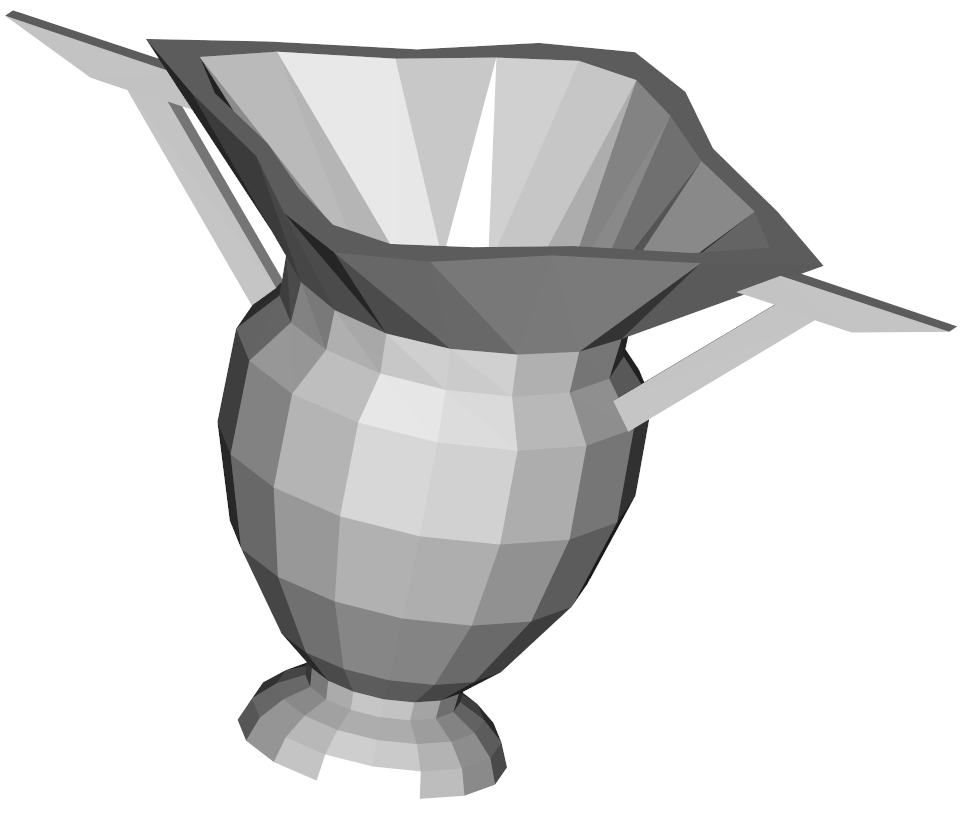
\includegraphics[width = \textwidth]{saffd_0.png}
		\caption{传统自由变形结果}\label{subfig:saffd_0}
	\end{subfigure}
	\quad
	\begin{subfigure}[b]{.3\textwidth}
		\centering
		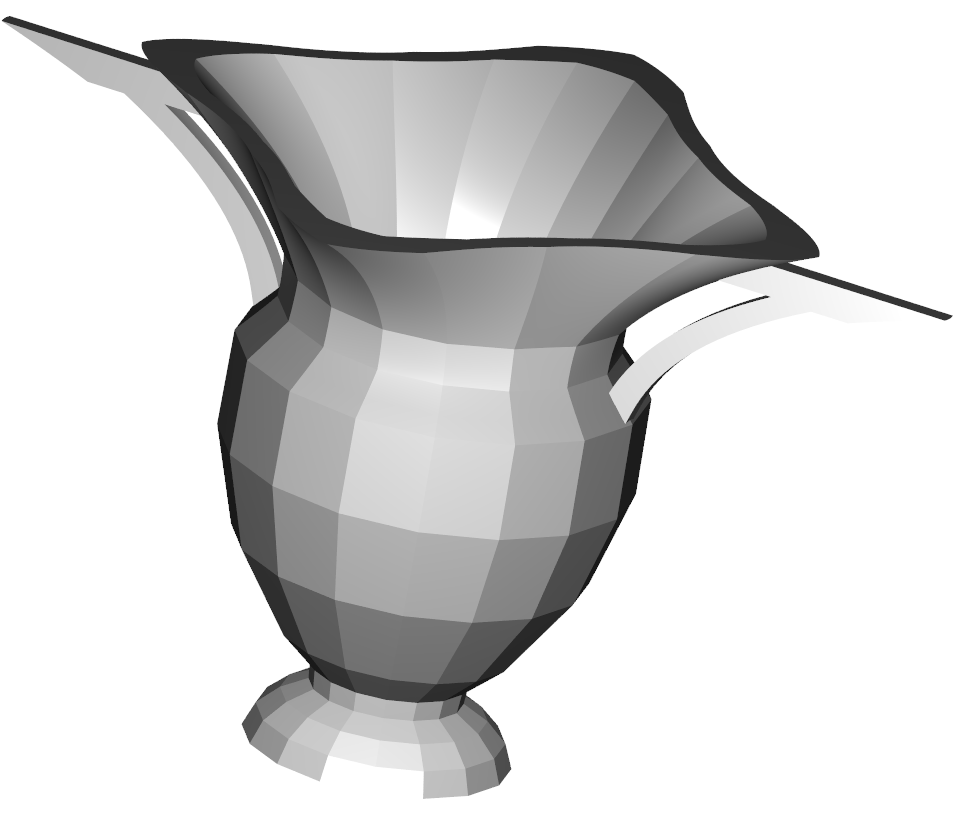
\includegraphics[width = \textwidth]{saffd_1.png}
		\caption{精确自由变形结果}\label{subfig:saffd_1}
	\end{subfigure}
	\quad
	\begin{subfigure}[b]{.3\textwidth}
		\centering
		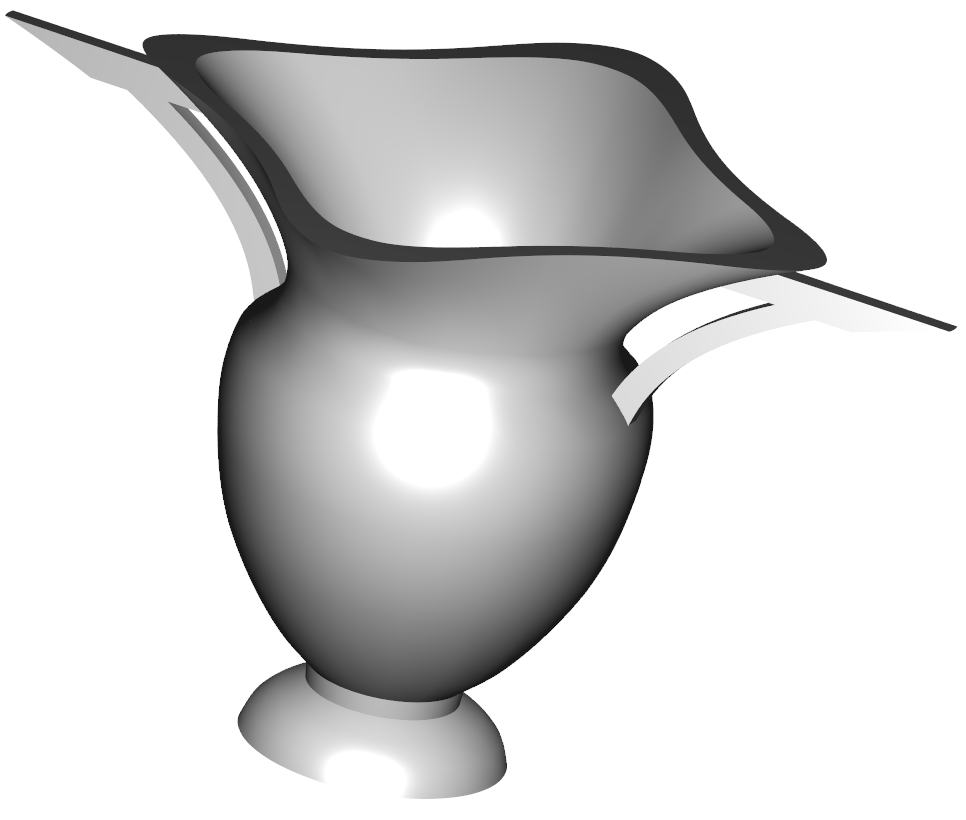
\includegraphics[width = \textwidth]{saffd_2.png}
		\caption{光滑自由变形结果}\label{subfig:saffd_2}
	\end{subfigure}
    \caption{传统自由变形、精确自由变形和光滑自由变形的结果对比}\label{fig:sample_problem_saffd}
\end{figure}


%自由变形(Free Form Deformation)是一类编辑几何模型、生成柔体性动画的方法。由于其实现简单,与模型表示无关,所以被广泛的应用于计算机辅助设计与工程、计算机动画、医学影影等领域。另一方面,由于其较强的可拓展性,FFD\cite{Sederberg86}自提出以来就受到了学术届的广泛关注,该工作不仅实现了一种具体的编辑三维模型的方法,更重要的是是提出了一套编辑三维模型的算法框架。研究人员在这一框架的基础上,做了很多工作。主要从算法效率、变形结果、交互方式三方面对FFD进行了改进:


%在FFD交互方式的探索中,研究者主要着眼于变形空间的选取。不同的变形空间,适用于不同的编辑需求,同时也会影响用户的交互方式。总体而言,用户编辑模型时可以控制的变量越多,算法对模型的编辑能力就越强,同时用户的交互也越复杂。


\section{本文内容安排}
本文的内容安排如下:
第一章介绍了本文研究背景,回顾了空间变形领域的相关工作。其中,重点介绍了自由变形的发展和局限。同时引出了本文希望解决的问题。

本文基于光滑自由变形,在此基础上对其中的“切割原始三角形”这一步骤进行了改进,并用OpenGL Compute实现了所有算法步骤,包括“切割原始三角形”,光滑自由变形的这一步骤是在CPU上实现的。除了以上两点改进。本文算法均与光滑自由变形一致。所以本文在第二章对光滑自由变形\cite{Cui15}的各个步骤进行了简单介绍。

第三章详细介绍了本文提出的新的三角形分割算法,并提出了参数$l$,用以控制原始面片被分割的粒度。还分析了参数$l$对算法效率、生成的子三角形的质量、变形结果的精度等方面的影响。

第四章介绍了算法的具体实现。算法将所有计算过程实现成了若干个OpenGL的Compute Shader,利用GPU的并行能力对提高了算法的运行速度,使用户能够交互的进行三维模型形状的编辑。新的三角形分割算法本身难以通过目前的GPU通用计算架构实现,所以我们提前计算不同的三角形的分割方案并储存起来,GPU分割三角形时直接通过三边比例找到合适的分割方案进行分割。同时,OpenGL作为跨平台通用的应用程序编程接口,给本文方法带来了良好的通用性。此外,本章还介绍了如何将新的三角形分割算法应用到Compute Shader中,使整个变形过程都在GPU中执行。

第五章讲述了本文算法在移动平台上的应用。我们实现了一个安卓平台上的模拟陶瓷制作过程的应用--哇陶。该应用可以让用户制作出个性化的瓷器。本文算法应用在泥胚塑形环节,以帮助用户得到满意的造型。

第六章对本文算法与光滑自由变形\cite{Cui15},精确自由变形\cite{Feng00}进行了多方面的对比,包括绘制效果、算法时间、变形精度等。

最后一章对本文工作进行了总结,概括了本文方法的优势与适用场景。还提出了本文方法的一些不足之处并对未来的研究工作进行了展望。




